\documentclass[14pt]{extarticle}
\usepackage[utf8]{inputenc}
\usepackage{tkz-euclide}
\usepackage{tikz} 
\usepackage{pdflscape}
\usepackage[margin=2cm]{geometry}
\usepackage{amsmath}

\begin{document}
\begin{center}
    \LARGE{\textbf{Esercitazione geometria Teorema Pitagora - 04/10/2022 - 3B}}
\end{center}
\vspace{1cm}

%----- FINE CONSEGNA -----
\textbf{Problema 1:} il triangolo \textit{ABC} in figura ha il lato \(\overline{CB}\) di 5cm e il lato \(\overline{AC}\) di 10 cm. Disegna sulla figura l'altezza relativa al lato \(\overline{CB}\), calcolane la lunghezza e calcola area e perimetro.

\vspace{0.5cm}
\begin{tikzpicture}[rotate=0]
    \tkzDefPoint(2,3){A}
    \tkzDefShiftPoint[A](0:4){B}
    \tkzDefShiftPoint[A](30:4){C}
    \tkzDefMidPoint(B,C)
    %\tkzGetPoint{H}
    \tkzDrawSegments(A,B B,C C,A)
    \tkzMarkSegments[mark=|](A,B A,C)
    \tkzDrawPoints(A,B,C)
    \tkzLabelPoints[above right](C)
    \tkzLabelPoints[right](B)
    \tkzLabelPoints[left](A)
    %\tkzDrawSegments[style=dashed](A,H)
\end{tikzpicture}

\vspace{0.5cm}
\textbf{Problema 2:} dai un nome alla figure rappresentata (aiutati con il righello). Sapendo che il lato \(\overline{BC}\) misura 3 cm, disegna una diagonale della figura e calcolane la lunghezza, infine calcola il perimetro e l'area.\\

\vspace{0.5cm}
%quadrato
\hspace{0.5cm}
\begin{tikzpicture}[scale=1, rotate=45]
    \tkzDefPoints{0/0/A,2/0/B,2/2/C,0/2/D}
    \tkzDrawPolygon(A,...,D)
    \tkzDrawPoints(A,...,D)
    \tkzLabelPoints[below](A)
    \tkzLabelPoints[left](D)
    \tkzLabelPoints[right](B)
    \tkzLabelPoints[above](C)
\end{tikzpicture}

\vspace{0.5cm}
\textbf{Problema 3:} nella figura la diagonale maggiore \(\overline{BD}\) misura \(8cm\) e la diagonale minore \(\overline{CA}\) misura \(\dfrac{1}{4}\) di \(\overline{BD}\). Calcolare area e perimetro.\\

%rombo
\hspace{0.5cm}
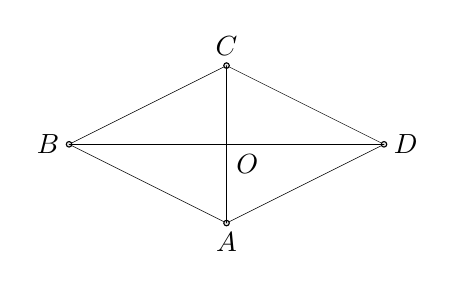
\begin{tikzpicture}[scale=1, rotate=0]
    \tkzDefPoints{2/0/A,4/1/D,0/1/B,2/2/C,2/1/O}
    \tkzDrawPolygon(A,...,D)
    \tkzDrawPoints(A,...,D)
    \tkzLabelPoints[below](A)
    \tkzLabelPoints[right](D)
    \tkzLabelPoints[left](B)
    \tkzLabelPoints[above](C)
    \tkzLabelPoints[below right](O)
    \tkzDrawSegments(A,C)
    \tkzDrawSegments(B,D)
\end{tikzpicture}

\clearpage
\textbf{Problema 4:} nella figura il lato \(\overline{CD}\) misura 3cm e la diagonale \(\overline{CA}\) misura 5 cm. Trova area e perimetro.\\

\vspace{0.5cm}
%quadrato
\hspace{0.5cm}
\begin{tikzpicture}[scale=1, rotate=45]
    \tkzDefPoints{0/0/A,2/0/B,2/4/C,0/4/D}
    \tkzDrawPolygon(A,...,D)
    \tkzDrawPoints(A,...,D)
    \tkzLabelPoints[below](A)
    \tkzLabelPoints[left](D)
    \tkzLabelPoints[right](B)
    \tkzLabelPoints[above](C)
    \tkzDrawSegments[style=dashed](A,C)
\end{tikzpicture}

\vspace{1cm}
\textbf{Problema 5:} l'area della figura misura \(24cm^2\), il lato \(\overline{AB}\) 10cm e il lato \(\overline{CD}\) 7cm. Calcola il perimetro. Disegna le diagonali della figura e calcolane la lunghezza.\\

\vspace{0.5cm}
\begin{tikzpicture}[scale=1, rotate=42]
    \tkzDefPoints{0/0/A,4/0/B,3/2/C,0/2/D}
    \tkzDrawPolygon(A,...,D)
    \tkzDrawPoints(A,...,D)
    \tkzDefMidPoint(B,C)
    \tkzDefPointBy[projection=onto B--A](C) \tkzGetPoint{H} %ALTEZZA
    \tkzDrawSegments[style=dashed](C,H)
    \tkzLabelPoints[left](D)
    \tkzLabelPoints[below](A)
    \tkzLabelPoints[above](C)
    \tkzLabelPoints[right](B)
    \tkzLabelPoints[below right](H)
\end{tikzpicture}

\vspace{1cm}
\textbf{Problema 6:} nella figura il lato \(\overline{DC}\) misura 6cm, il segmento \(\overline{AH}\) è \(\dfrac{1}{3}\) del lato \(\overline{AB}\). Se l'area è \(40cm^2\) quanto vale il perimetro?\\

\vspace{0.5cm}
\begin{tikzpicture}[scale=1.1]
    %initialisation
    \tkzInit[xmin=0,xmax=4,ymin=0,ymax=2] 
    \tkzClip[space=.5] 
    %definitions
    \tkzDefPoint(0,0){A} 
    \tkzDefPoint(3,0){B} 
    \tkzDefPoint(4,2){C} 
    \tkzDefPoint(1,0){H}
    \tkzDefPointWith[colinear= at C](B,A) \tkzGetPoint{D}
    %drawing
    \tkzDrawPolygon(A,B,C,D)
    %\tkzDrawSegments[blue,dashed](A,C B,D)
    %label
    \tkzLabelPoints[below](A,B,H)
    \tkzLabelPoints[above](C,D)
    \tkzDrawSegments[style=dashed](D,H)
    %\tkzLabelSegment[above,pos=.7,sloped](A,C){$x+y$}
    %\tkzLabelSegme
\end{tikzpicture}
\clearpage

%-------SOLUZIONI

\begin{center}\textbf{Soluzioni}\end{center}

\textbf{Problema 1:}\\
L'altezza relativa al lato \(\overline{CB}\) di questo \textit{TRIANGOLO ISOSCELE} è un segmento che parte dal vertice \(A\) e cade perpendicolarmente sul lato \(\overline{CB}\). Per calcolare la lunghezza dell'altezza si può utilizzare il Teorema di Pitagora considerando metà della base \(\overline{CB}\) e uno dei due lati (\(\overline{AB}\) o \(\overline{CA}\)) (Nella figura triangolo segnato di rosso) \\
\begin{center}
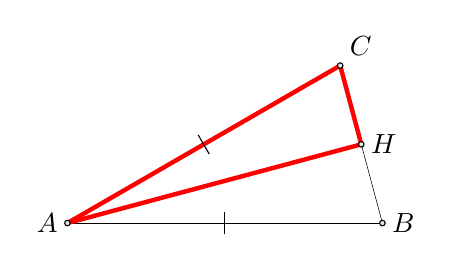
\begin{tikzpicture}[rotate=0]
    \tkzDefPoint(2,3){A}
    \tkzDefShiftPoint[A](0:4){B}
    \tkzDefShiftPoint[A](30:4){C}
    \tkzDefMidPoint(B,C)
    \tkzGetPoint{H}
    \tkzDrawSegments(A,B B,H)
    \tkzDrawSegments[color=red,ultra thick](C,A C,H A,H)
    \tkzMarkSegments[mark=|](A,B A,C)
    \tkzDrawPoints(A,B,C,H)
    \tkzLabelPoints[above right](C)
    \tkzLabelPoints[right](B)
    \tkzLabelPoints[left](A)
    \tkzLabelPoints[right](H)
    %\tkzDrawSegments[style=dashed](A,H)
\end{tikzpicture}
\end{center}
Quindi:
\[\overline{AH}=\sqrt[2]{\overline{AC}^2-\overline{CH}^2}=\sqrt[2]{(10cm)^2-(2,5cm)^2}=\]\[=\sqrt[2]{100cm^2-6,25cm^2}=\sqrt[2]{93,75cm^2}\approx9,68cm\]
Calcolata l'altezza si può ricavare l'area applicando la formula:
\[area=\dfrac{base\cdot altezza}{2}=\dfrac{\overline{BC}\cdot\overline{AH}}{2}=\dfrac{5cm\cdot9,68cm}{2}=\dfrac{48,4cm^2}{2}=24,24cm^2\] 
Infine si può ottenere il perimetro sommando i 3 lati:
\[2p=\overline{AB}+\overline{BC}+\overline{CA}=10cm+10cm+5cm=10cm\cdot2+5cm=25cm\]

\textbf{Problema 2:}\\
La figura è un \textit{quadrato} (tutti i lati sono uguali e perpendicolari tra di loro (formano angoli di 90°)). Le diagonali in un quadrato sono 2, per la consegna del problema basta disegnarne una. Nella figura seguente le diagonali sono una rossa e una blu:\\
\hspace{0.5cm}
\begin{center}
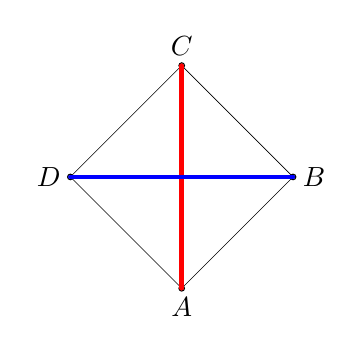
\begin{tikzpicture}[scale=1, rotate=45]
    \tkzDefPoints{0/0/A,2/0/B,2/2/C,0/2/D}
    \tkzDrawPolygon(A,...,D)
    \tkzDrawPoints(A,...,D)
    \tkzDrawSegments[color=red,ultra thick](C,A)
    \tkzDrawSegments[color=blue,ultra thick](D,B)
    \tkzLabelPoints[below](A)
    \tkzLabelPoints[left](D)
    \tkzLabelPoints[right](B)
    \tkzLabelPoints[above](C)
\end{tikzpicture}
\end{center}
Per trovare la lunghezza della diagonale si può utilizzare il teorema di Pitagora considerando diversi triangoli all'interno del quadrato:
\hspace{0.5cm}
\begin{center}
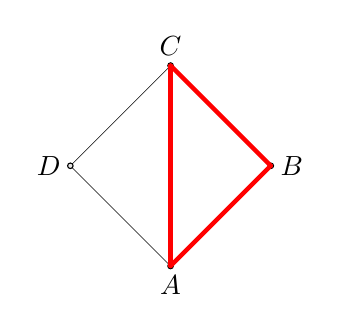
\begin{tikzpicture}[scale=0.9, rotate=45]
    \tkzDefPoints{0/0/A,2/0/B,2/2/C,0/2/D}
    \tkzDrawPolygon(A,...,D)
    \tkzDrawPoints(A,...,D)
    \tkzDrawSegments[color=red,ultra thick](C,A C,B B,A)
    \tkzLabelPoints[below](A)
    \tkzLabelPoints[left](D)
    \tkzLabelPoints[right](B)
    \tkzLabelPoints[above](C)
\end{tikzpicture}
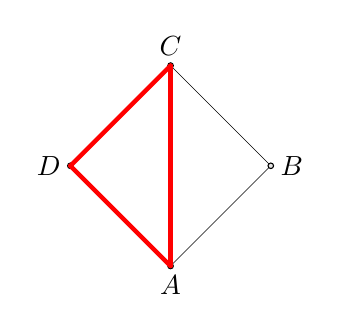
\begin{tikzpicture}[scale=0.9, rotate=45]
    \tkzDefPoints{0/0/A,2/0/B,2/2/C,0/2/D}
    \tkzDrawPolygon(A,...,D)
    \tkzDrawPoints(A,...,D)
    \tkzDrawSegments[color=red,ultra thick](C,A C,D D,A)
    \tkzLabelPoints[below](A)
    \tkzLabelPoints[left](D)
    \tkzLabelPoints[right](B)
    \tkzLabelPoints[above](C)Esercitazione geometria Teorema
\end{tikzpicture}
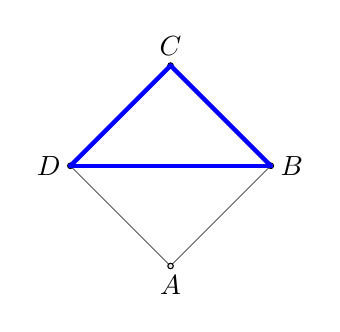
\begin{tikzpicture}[scale=0.9, rotate=45]
    \tkzDefPoints{0/0/A,2/0/B,2/2/C,0/2/D}
    \tkzDrawPolygon(A,...,D)
    \tkzDrawPoints(A,...,D)
    \tkzDrawSegments[color=blue,ultra thick](D,B D,C B,C)
    \tkzLabelPoints[below](A)
    \tkzLabelPoints[left](D)
    \tkzLabelPoints[right](B)
    \tkzLabelPoints[above](C)
\end{tikzpicture}
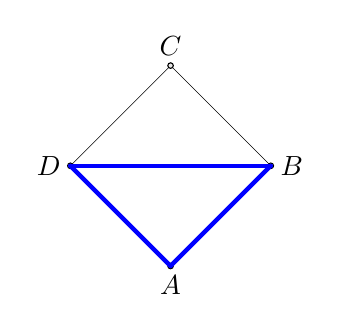
\begin{tikzpicture}[scale=0.9, rotate=45]
    \tkzDefPoints{0/0/A,2/0/B,2/2/C,0/2/D}
    \tkzDrawPolygon(A,...,D)
    \tkzDrawPoints(A,...,D)
    \tkzDrawSegments[color=blue,ultra thick](D,B D,A B,A)
    \tkzLabelPoints[below](A)
    \tkzLabelPoints[left](D)
    \tkzLabelPoints[right](B)
    \tkzLabelPoints[above](C)
\end{tikzpicture}
\end{center}
Prendendo come esempio il primo quadrato a sinistra risulta che i lati \(\overline{AB}\) e \(\overline{CB}\) sono i cateti del triangolo rettangolo (evidenziato in rosso) e la diagonale \(\overline{CA}\) del quadrato \(ABCD\) è l'ipotenusa del triangolo stesso. Quindi si può calcolare la lunghezza del lato \(\overline{CA}\) come seguente:

\[\overline{CA}=\sqrt[2]{\overline{AB}^2+\overline{BC}^2}=\sqrt[2]{(3cm)^2+(3cm)^2}=\sqrt[2]{18cm}\]

il numero 18 può essere visto come \(9\cdot2\) e il numero 9 può essere considerato come \(3^2\), quindi \(\sqrt[2]{18}\) si può riscrivere come:

\[\sqrt[2]{18cm}=\sqrt[2]{9cm\cdot2}=\sqrt[2]{(3cm)^2\cdot2}\]

applicando la proprietà delle potenze \(\sqrt[2]{a\cdot b}=\sqrt[2]{a}\cdot\sqrt[2]{b}\) si può riscrivere l'uguaglianza precedente come:

\[\sqrt[2]{18cm}=\sqrt[2]{(3cm)^2\cdot2}=\sqrt[2]{(3cm)^2}\cdot\sqrt[2]{2}=3cm\cdot\sqrt[2]{2}\] 

che è proprio la dimostrazione che una diagonale del quadrato si può trovare applicando direttamente la formula \(diagonale=l\cdot\sqrt[2]{2}\).\\
Il 2p si trova semplicemente sommando i 4 lati (o moltiplicando un lato per 4 volte):

\[2p=3cm\cdot4=16cm\]
mentre per l'area si applica la formula \(l\cdot l\):
\[area=l\cdot l=3cm\cdot 3cm=9cm^2\]

\textbf{Problema 3:}\\
La figura è un \textit{ROMBO} e l'area si calcola mediante la formula:
\[area=\dfrac{Dmag\cdot Dmin}{2}=\dfrac{\overline{BD}\cdot\overline{CA}}{2}\]

dove \(Dmag\) è la diagonale maggiore e \(Dmin\) è la digonale minore. Per calcolarsi \(Dmin\) si applica l'uguaglianza fornita dal probema:
\[\overline{CA}=\dfrac{1}{4}\overline{BD}=\dfrac{1}{4}\cdot{8cm}=\dfrac{1\cdot 8cm}{4}=2cm\]

quindi:
\[area=\dfrac{\overline{BD}\cdot\overline{CA}}{2}=\dfrac{8cm\cdot 2cm}{2}= \dfrac{16cm^2}{2}=8cm^2\]

per calcolare il perimetro bisogna trovare la lunghezza di un lato e moltiplicarlo per i 4 lati. La lunghezza del lato non è nota ma si può calcolare attraverso il teorema di Pitagora considerando uno dei 4 triangoli rettangoli presenti in figura in cui l'ipotenusa è il lato del rombo:\\
\hspace{0.5cm}
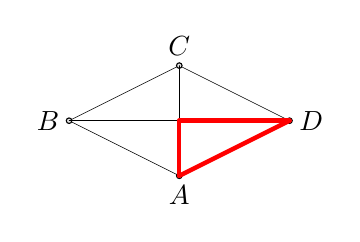
\begin{tikzpicture}[scale=0.7, rotate=0]
    \tkzDefPoints{2/0/A,4/1/D,0/1/B,2/2/C,2/1/O}
    \tkzDrawPolygon(A,...,D)
    \tkzDrawPoints(A,...,D)
    \tkzLabelPoints[below](A)
    \tkzLabelPoints[right](D)
    \tkzLabelPoints[left](B)
    \tkzLabelPoints[above](C)
    \tkzDrawSegments(A,C)
    \tkzDrawSegments(B,D)
    \tkzDrawSegments[color=red,ultra thick](A,D D,O O,A)
\end{tikzpicture}
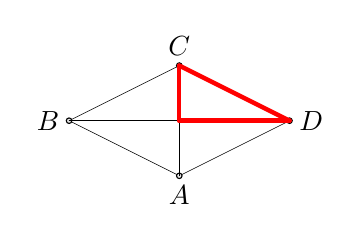
\begin{tikzpicture}[scale=0.7, rotate=0]
    \tkzDefPoints{2/0/A,4/1/D,0/1/B,2/2/C,2/1/O}
    \tkzDrawPolygon(A,...,D)
    \tkzDrawPoints(A,...,D)
    \tkzLabelPoints[below](A)
    \tkzLabelPoints[right](D)
    \tkzLabelPoints[left](B)
    \tkzLabelPoints[above](C)
    \tkzDrawSegments(A,C)
    \tkzDrawSegments(B,D)
    \tkzDrawSegments[color=red,ultra thick](C,D C,O O,D)
\end{tikzpicture}
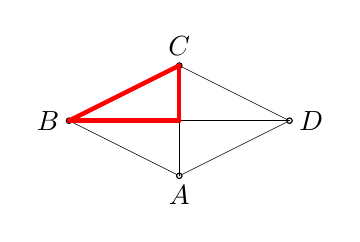
\begin{tikzpicture}[scale=0.7, rotate=0]
    \tkzDefPoints{2/0/A,4/1/D,0/1/B,2/2/C,2/1/O}
    \tkzDrawPolygon(A,...,D)
    \tkzDrawPoints(A,...,D)
    \tkzLabelPoints[below](A)
    \tkzLabelPoints[right](D)
    \tkzLabelPoints[left](B)
    \tkzLabelPoints[above](C)
    \tkzDrawSegments(A,C)
    \tkzDrawSegments(B,D)
    \tkzDrawSegments[color=red,ultra thick](C,B C,O O,B)
\end{tikzpicture}
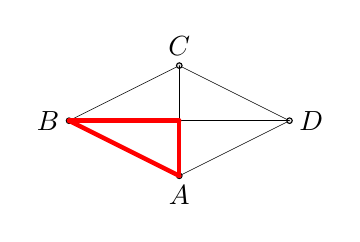
\begin{tikzpicture}[scale=0.7, rotate=0]
    \tkzDefPoints{2/0/A,4/1/D,0/1/B,2/2/C,2/1/O}
    \tkzDrawPolygon(A,...,D)
    \tkzDrawPoints(A,...,D)
    \tkzLabelPoints[below](A)
    \tkzLabelPoints[right](D)
    \tkzLabelPoints[left](B)
    \tkzLabelPoints[above](C)
    \tkzDrawSegments(A,C)
    \tkzDrawSegments(B,D)
    \tkzDrawSegments[color=red,ultra thick](A,B A,O O,B)
\end{tikzpicture}

Per sapere la lunghezza dei cateti di ogni triangolino interno al rombo bisogna ricordarsi la proprietà del rombo che dice che le diagonali si dividono a metà, quindi la metà di ogni diagonale sarà il cateto (maggiore o minore) di ogni triangolo rettangolo disegnato in rosso.\\
Quindi il lato del rombo si trova:\\
\[lato=\sqrt[2]{(\dfrac{1}{2}\cdot8cm)^2+(\dfrac{1}{2}\cdot4cm)^2}=\sqrt[2]{(4cm)^2+(2cm)^2}=\sqrt[2]{16cm^2+4cm^2}=\]
\[=\sqrt[2]{20cm^2}=\sqrt[2]{20}cm\]
e di conseguenza il perimetro:
\[2p=\sqrt[2]{20}cm+\sqrt[2]{20}cm+\sqrt[2]{20}cm+\sqrt[2]{20}cm=\sqrt[2]{20}cm\cdot 4=4\sqrt[2]{20}cm\]

\textbf{Problema 4:}\\
Nel problema viene fornita la lunghezza del lato \(\overline{CD}\) (uno dei due lati minori del rettangolo) e della diagonale \(\overline{CA}\). Per trovare il perimetro e l'area abbiamo bisogno di conoscere la misura di uno dei lati più lunghi del rettangolo (o il lato \(\overline{DA}\) o il lato \(\overline{CB}\).\\
Se consideriamo il triangolo rettangolo \(CDA\) abbiamo già il cateto minore \(\overline{CD}\) e l'ipotenusa \(\overline{CA}\):\\
\hspace{0.5cm}
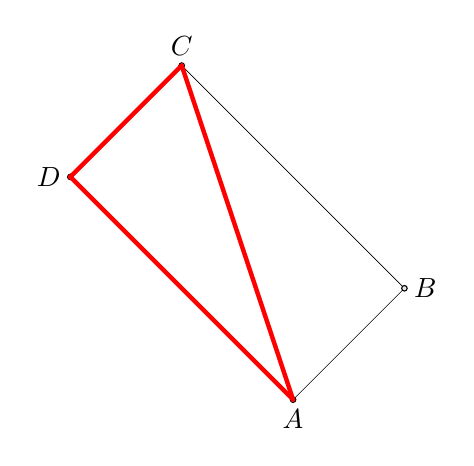
\begin{tikzpicture}[scale=1, rotate=45]
    \tkzDefPoints{0/0/A,2/0/B,2/4/C,0/4/D}
    \tkzDrawPolygon(A,...,D)
    \tkzDrawPoints(A,...,D)
    \tkzLabelPoints[below](A)
    \tkzLabelPoints[left](D)
    \tkzLabelPoints[right](B)
    \tkzLabelPoints[above](C)
    \tkzDrawSegments[color=red,ultra thick](A,C)
    \tkzDrawSegments[color=red,ultra thick](D,C)
    \tkzDrawSegments[color=red,ultra thick](A,D)
\end{tikzpicture}\\
quindi possiamo applicare il teorema di Pitagora per ricavare il cateto maggiore avendo il cateto minore e l'ipotenusa:\\
\[\overline{DA}=\sqrt[2]{Ipot^2-Cmin^2}=\sqrt[2]{\overline{CA}^2-\overline{CD}^2}=\sqrt[2]{(5cm)^2-(3cm)^2}=\]\[=\sqrt[2]{25cm^2-9cm^2}=\sqrt[2]{16m^2}=\sqrt[2]{4^2cm^2}=4cm\]
Calcolato il lato maggiore è semplice trovare sia il perimetro che l'area:
\[2p=\overline{CD}\cdot2+\overline{DA}\cdot2=4cm\cdot2+3cm \cdot2=8cm+6cm=14cm\]
\[area=\overline{DA}\cdot\overline{CD}=4cm\cdot3cm=12cm^2\]

\textbf{Problema 5:}\\
Il \textit{TRAPEZIO RETTANGOLO} ha due diagonali:\\
\vspace{0.5cm}
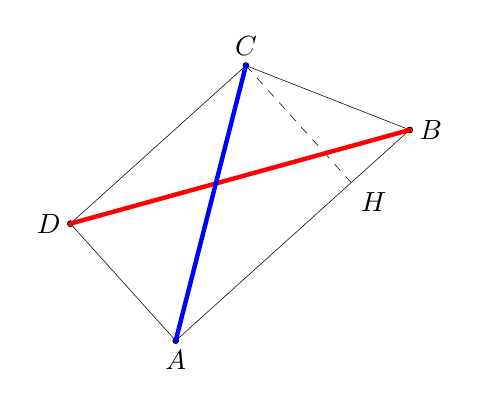
\begin{tikzpicture}[scale=1, rotate=42]
    \tkzDefPoints{0/0/A,4/0/B,3/2/C,0/2/D}
    \tkzDrawPolygon(A,...,D)
    \tkzDrawPoints(A,...,D)
    \tkzDefMidPoint(B,C)
    \tkzDefPointBy[projection=onto B--A](C) \tkzGetPoint{H} %ALTEZZA
    \tkzDrawSegments[style=dashed](C,H)
    \tkzLabelPoints[left](D)
    \tkzLabelPoints[below](A)
    \tkzLabelPoints[above](C)
    \tkzLabelPoints[right](B)
    \tkzLabelPoints[below right](H)
    \tkzDrawSegments[color=red,ultra thick](D,B)
    \tkzDrawSegments[color=blue,ultra thick](A,C)
\end{tikzpicture}

queste due diagonali possono essere considerate ipotenuse di diversi triangoli rettangoli "interni" al trapezio rettangolo:\vspace{0.5cm}\\

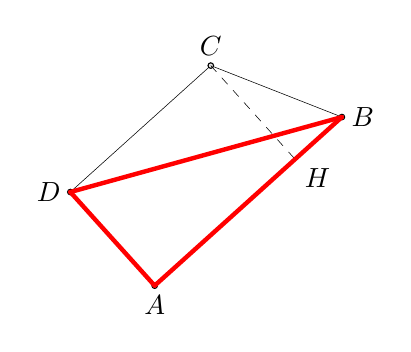
\begin{tikzpicture}[scale=0.8, rotate=42]
    \tkzDefPoints{0/0/A,4/0/B,3/2/C,0/2/D}
    \tkzDrawPolygon(A,...,D)
    \tkzDrawPoints(A,...,D)
    \tkzDefMidPoint(B,C)
    \tkzDefPointBy[projection=onto B--A](C) \tkzGetPoint{H} %ALTEZZA
    \tkzDrawSegments[style=dashed](C,H)
    \tkzLabelPoints[left](D)
    \tkzLabelPoints[below](A)
    \tkzLabelPoints[above](C)
    \tkzLabelPoints[right](B)
    \tkzLabelPoints[below right](H)
    \tkzDrawSegments[color=red,ultra thick](D,B)
    \tkzDrawSegments[color=red,ultra thick](D,A)
    \tkzDrawSegments[color=red,ultra thick](A,B)
\end{tikzpicture}
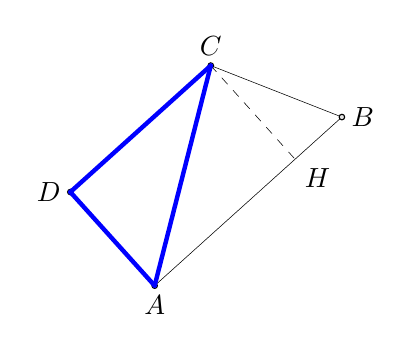
\begin{tikzpicture}[scale=0.8, rotate=42]
    \tkzDefPoints{0/0/A,4/0/B,3/2/C,0/2/D}
    \tkzDrawPolygon(A,...,D)
    \tkzDrawPoints(A,...,D)
    \tkzDefMidPoint(B,C)
    \tkzDefPointBy[projection=onto B--A](C) \tkzGetPoint{H} %ALTEZZA
    \tkzDrawSegments[style=dashed](C,H)
    \tkzLabelPoints[left](D)
    \tkzLabelPoints[below](A)
    \tkzLabelPoints[above](C)
    \tkzLabelPoints[right](B)
    \tkzLabelPoints[below right](H)
    \tkzDrawSegments[color=blue,ultra thick](C,A)
    \tkzDrawSegments[color=blue,ultra thick](D,C)
    \tkzDrawSegments[color=blue,ultra thick](A,D)
\end{tikzpicture}\\
oppure anche triangoli non rettangoli ma che possono capitare in alcuni problemi (sopratutto quello verde, mentre quello giallo è più difficile):\vspace{0.5cm}\\
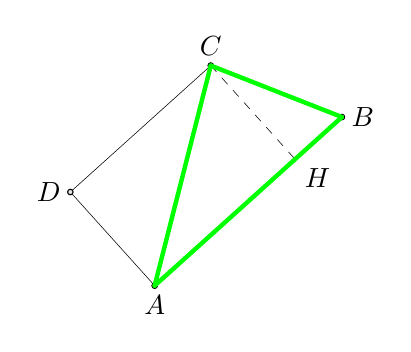
\begin{tikzpicture}[scale=0.8, rotate=42]
    \tkzDefPoints{0/0/A,4/0/B,3/2/C,0/2/D}
    \tkzDrawPolygon(A,...,D)
    \tkzDrawPoints(A,...,D)
    \tkzDefMidPoint(B,C)
    \tkzDefPointBy[projection=onto B--A](C) \tkzGetPoint{H} %ALTEZZA
    \tkzDrawSegments[style=dashed](C,H)
    \tkzLabelPoints[left](D)
    \tkzLabelPoints[below](A)
    \tkzLabelPoints[above](C)
    \tkzLabelPoints[right](B)
    \tkzLabelPoints[below right](H)
    \tkzDrawSegments[color=green,ultra thick](C,A)
    \tkzDrawSegments[color=green,ultra thick](B,C)
    \tkzDrawSegments[color=green,ultra thick](A,B)
\end{tikzpicture}
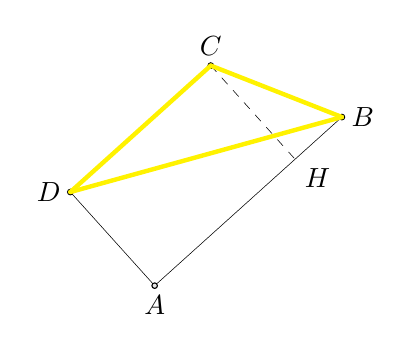
\begin{tikzpicture}[scale=0.8, rotate=42]
    \tkzDefPoints{0/0/A,4/0/B,3/2/C,0/2/D}
    \tkzDrawPolygon(A,...,D)
    \tkzDrawPoints(A,...,D)
    \tkzDefMidPoint(B,C)
    \tkzDefPointBy[projection=onto B--A](C) \tkzGetPoint{H} %ALTEZZA
    \tkzDrawSegments[style=dashed](C,H)
    \tkzLabelPoints[left](D)
    \tkzLabelPoints[below](A)
    \tkzLabelPoints[above](C)
    \tkzLabelPoints[right](B)
    \tkzLabelPoints[below right](H)
    \tkzDrawSegments[color=yellow,ultra thick](D,B)
    \tkzDrawSegments[color=yellow,ultra thick](D,C)
    \tkzDrawSegments[color=yellow,ultra thick](C,B)
\end{tikzpicture}\\
Avendo l'area della figura, la base maggiore e la base minore forniti dal problema si può ricavare l'altezza:
\[area=\dfrac{(Bmag+Bmin)\cdot h}{2}\]
quindi l'altezza:
\[h=\dfrac{area\cdot 2}{(Bmag+Bmin)}=\dfrac{24cm^2\cdot 2}{(10cm+7cm)}=\dfrac{48cm^2}{17cm}\approx2,82cm=\overline{CH}=\overline{DA}\]
Per calcolare la diagonale \(\overline{DB}\) si può considerare il triangolo \(DAB\):\\
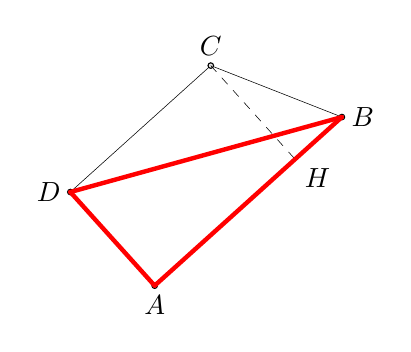
\begin{tikzpicture}[scale=0.8, rotate=42]
    \tkzDefPoints{0/0/A,4/0/B,3/2/C,0/2/D}
    \tkzDrawPolygon(A,...,D)
    \tkzDrawPoints(A,...,D)
    \tkzDefMidPoint(B,C)
    \tkzDefPointBy[projection=onto B--A](C) \tkzGetPoint{H} %ALTEZZA
    \tkzDrawSegments[style=dashed](C,H)
    \tkzLabelPoints[left](D)
    \tkzLabelPoints[below](A)
    \tkzLabelPoints[above](C)
    \tkzLabelPoints[right](B)
    \tkzLabelPoints[below right](H)
    \tkzDrawSegments[color=red,ultra thick](D,B)
    \tkzDrawSegments[color=red,ultra thick](D,A)
    \tkzDrawSegments[color=red,ultra thick](A,B)
\end{tikzpicture}\\
e facendo il teorema di Pitagora tra il lato \(DA\) (congruente all'altezza del trapezio) e il lato \(\overline{AB}\) (Base maggiore) si ottiene:\\
\[\overline{DB}=\sqrt[2]{\overline{AD}^2+\overline{AB}^2}=\sqrt[2]{(2,82cm)^2+(10cm)^2}=\]\[=\sqrt[2]{7,95cm^2+100cm^2}=\sqrt[2]{107,95cm^2}\approx10,39cm\]
per calcolare invece la diagonale \(\overline{CA}\) si può in maniera simile:\\
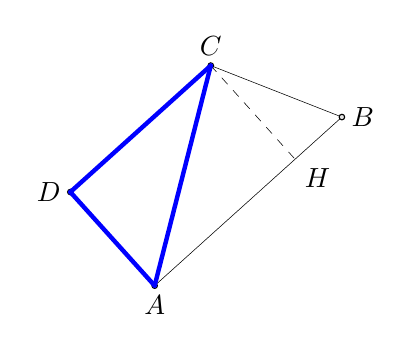
\begin{tikzpicture}[scale=0.8, rotate=42]
    \tkzDefPoints{0/0/A,4/0/B,3/2/C,0/2/D}
    \tkzDrawPolygon(A,...,D)
    \tkzDrawPoints(A,...,D)
    \tkzDefMidPoint(B,C)
    \tkzDefPointBy[projection=onto B--A](C) \tkzGetPoint{H} %ALTEZZA
    \tkzDrawSegments[style=dashed](C,H)
    \tkzLabelPoints[left](D)
    \tkzLabelPoints[below](A)
    \tkzLabelPoints[above](C)
    \tkzLabelPoints[right](B)
    \tkzLabelPoints[below right](H)
    \tkzDrawSegments[color=blue,ultra thick](C,A)
    \tkzDrawSegments[color=blue,ultra thick](D,C)
    \tkzDrawSegments[color=blue,ultra thick](A,D)
\end{tikzpicture}\\
\[\overline{CA}=\sqrt[2]{\overline{CD}^2+\overline{DA}^2}=\sqrt[2]{(7cm)^2+(2,82cm)^2}=\]\[=\sqrt[2]{49cm^2+7,95cm^2}=\sqrt[2]{56,95cm^2}=7,55cm\]
\textbf{Problema 6:}\\
Nel parallelogramma in figura conosciamo l'area e i lati maggiori, quindi possiamo calcolarci l'altezza:\\
\[area=base\cdot altezza\]
\[altezza=\dfrac{area}{base}\]
\[\overline{DH}=\dfrac{40cm^2}{6cm}=6,7cm\]
visto che conosciamo la misura del segmento \(\overlin{AH}\) in relazione a \(\overlin{AB}\) lo possiamo calcolare:
\[\overline{AH}=\dfrac{1}{3}\overline{AB}=\dfrac{1}{3}6cm=2cm\]
se consideriamo il triangolo rettangolo in figura\vspace{0.5cm}\\

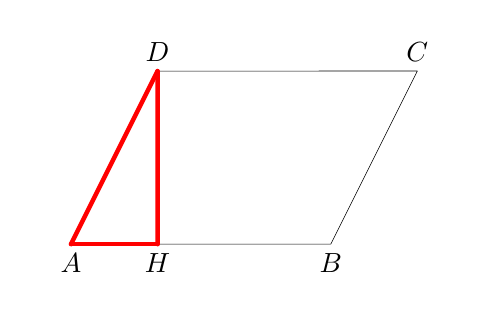
\begin{tikzpicture}[scale=1.1]
    %initialisation
    \tkzInit[xmin=0,xmax=4,ymin=0,ymax=2] 
    \tkzClip[space=.5] 
    %definitions
    \tkzDefPoint(0,0){A} 
    \tkzDefPoint(3,0){B} 
    \tkzDefPoint(4,2){C} 
    \tkzDefPoint(1,0){H}
    \tkzDefPointWith[colinear= at C](B,A) \tkzGetPoint{D}
    %drawing
    \tkzDrawPolygon(A,B,C,D)
    %\tkzDrawSegments[blue,dashed](A,C B,D)
    %label
    \tkzLabelPoints[below](A,B,H)
    \tkzLabelPoints[above](C,D)
    \tkzDrawSegments[style=dashed](D,H)
    \tkzDrawSegments[color=red,ultra thick](A,H)
    \tkzDrawSegments[color=red,ultra thick](D,H)
    \tkzDrawSegments[color=red,ultra thick](D,A)
    %\tkzLabelSegment[above,pos=.7,sloped](A,C){$x+y$}
    %\tkzLabelSegme
\end{tikzpicture}\\
Possiamo facilmente calcolare il lato \(\overline{DA}\) considerandolo come ipotenusa del triangolo \(ADH\):
\[\overline{AD}=\sqrt[2]{\overline{AH}^2+\overline{DH}^2}=\sqrt[2]{(2cm^2)+(6,7cm^2)}=\sqrt[2]{48,89cm^2}\approx7cm\]
Quindi il perimetro:
\[2p=\overline{AD}\cdot2+\overline{DC}\cdot2=7cm\cdot2+6cm\cdot2=26cm\]




\end{document}


